\section*{Výsledky měření}
Úspěšně jsme seřídili goniometr.
Používali jsme hranol č. 3 a lámavý úhel byl v rohu č. 2.
Používali jsme tekutinu č. 4.

Změřili jsme úhel normál obou přilehlých stěn pro hranol i kyvetu. Pro hranol byly údaje na goniometru \uhel{123}{0}{0} resp. \uhel{243}{9}{38}, pro kyvetu \uhel{107}{6}{24} resp. \uhel{226}{41}{30}. Podle \eqref{e:vrchol} určíme lámavý úhel hranolu $\varphi_h$ a kyvety $\varphi_k$
\begin{equation*}
\varphi_h = \uhel{59}{50}{22} \qquad \qquad \varphi_k = \uhel{60}{24}{54}
\end{equation*}



Změřili jsme indexy lomu čar spektra rtuťové výbojky v skleněném hranolu a kyvetě s tekutinou. Naměřené hodnoty jsou v tabulce \ref{t:uhly} a grafech \ref{g:h} a \ref{g:k}.


Měření jsme provedli víckrát a podle výsledků odhadujeme standardní chybu $\sigma_\delta = \sigma_\varphi = \uhel{0}{0}{30}$. Standardní odchylka indexu lomu vychází podle \eqref{e:chyba} pro všechny hodnoty $\sigma_n=\num{0.0001}$. Tato metoda zaručuje 3 číslice za desetinnou čárkou (4 platné číslice).


\begin{tabulka}[htbp]
\centering
\begin{tabular}{c||ccc|ccc}
 & \multicolumn{3}{c|}{skleněný hranol} & \multicolumn{3}{c}{kyveta s tekutinou} \\
$\lambda$ (\si{\nm}) & $\alpha_1$ & $\alpha_2$ & $n$ & $\alpha_1$ & $\alpha_2$ & $n$ \\ \hline
\num{404.7} & \uhel{203}{44}{14} & \uhel{124}{7}{10} & \num{1.5250} & \uhel{187}{56}{36} & \uhel{139}{41}{28} & \num{1.3411} \\ %a
\num{407.8} & \uhel{203}{41}{48} & \uhel{124}{9}{48} & \num{1.5246} & \uhel{187}{55}{20} & \uhel{139}{42}{16} & \num{1.3408} \\ %a
\num{435.8} & \uhel{203}{32}{18} & \uhel{124}{26}{36} & \num{1.5221} & \uhel{187}{44}{40} & \uhel{139}{52}{36} & \num{1.3386} \\ %a
\num{491.6} & \uhel{203}{8}{8} & \uhel{124}{52}{0} & \num{1.5175} & \uhel{187}{29}{24} & \uhel{140}{8}{10} & \num{1.3352} \\ %a
\num{546.1} & \uhel{202}{41}{58} & \uhel{125}{10}{0} & \num{1.5134} & \uhel{187}{18}{22} & \uhel{140}{18}{38} & \num{1.3329} \\ %a
\num{577.0} & \uhel{202}{34}{12} & \uhel{125}{17}{10} & \num{1.5120} & \uhel{187}{13}{20} & \uhel{140}{23}{40} & \num{1.3318} \\ %a
\num{579.1} & \uhel{202}{33}{42} & \uhel{125}{17}{50} & \num{1.5119} & \uhel{187}{13}{12} & \uhel{140}{24}{6} & \num{1.3317} \\ %a
\num{607.3} & \uhel{202}{27}{22} & \uhel{125}{23}{40} & \num{1.5107} & \uhel{187}{10}{0} & \uhel{140}{27}{42} & \num{1.3310} \\ %a
\num{612.3} & \uhel{202}{26}{26} & \uhel{125}{24}{26} & \num{1.5106} & \uhel{187}{8}{34} & \uhel{140}{28}{42} & \num{1.3307} \\ %a
\num{623.4} & \uhel{202}{24}{24} & \uhel{125}{26}{52} & \num{1.5102} & \uhel{187}{7}{16} & \uhel{140}{30}{0} & \num{1.3304} \\ %a
\num{671.6} & \uhel{202}{15}{48} & \uhel{125}{35}{24} & \num{1.5085} & \uhel{187}{1}{30} & \uhel{140}{35}{30} & \num{1.3292} \\ %a
\num{690.7} & \uhel{202}{13}{10} & \uhel{125}{38}{2} & \num{1.5080} & \uhel{186}{59}{34} & \uhel{140}{37}{48} & \num{1.3287} \\ %a

\end{tabular}
\caption{Indexy lomu spektrálních čar rtuťové výbojky}
\label{t:uhly}
\end{tabulka}


\begin{graph}
  \centering
  % GNUPLOT: LaTeX picture with Postscript
\begingroup
  \makeatletter
  \providecommand\color[2][]{%
    \GenericError{(gnuplot) \space\space\space\@spaces}{%
      Package color not loaded in conjunction with
      terminal option `colourtext'%
    }{See the gnuplot documentation for explanation.%
    }{Either use 'blacktext' in gnuplot or load the package
      color.sty in LaTeX.}%
    \renewcommand\color[2][]{}%
  }%
  \providecommand\includegraphics[2][]{%
    \GenericError{(gnuplot) \space\space\space\@spaces}{%
      Package graphicx or graphics not loaded%
    }{See the gnuplot documentation for explanation.%
    }{The gnuplot epslatex terminal needs graphicx.sty or graphics.sty.}%
    \renewcommand\includegraphics[2][]{}%
  }%
  \providecommand\rotatebox[2]{#2}%
  \@ifundefined{ifGPcolor}{%
    \newif\ifGPcolor
    \GPcolorfalse
  }{}%
  \@ifundefined{ifGPblacktext}{%
    \newif\ifGPblacktext
    \GPblacktexttrue
  }{}%
  % define a \g@addto@macro without @ in the name:
  \let\gplgaddtomacro\g@addto@macro
  % define empty templates for all commands taking text:
  \gdef\gplbacktext{}%
  \gdef\gplfronttext{}%
  \makeatother
  \ifGPblacktext
    % no textcolor at all
    \def\colorrgb#1{}%
    \def\colorgray#1{}%
  \else
    % gray or color?
    \ifGPcolor
      \def\colorrgb#1{\color[rgb]{#1}}%
      \def\colorgray#1{\color[gray]{#1}}%
      \expandafter\def\csname LTw\endcsname{\color{white}}%
      \expandafter\def\csname LTb\endcsname{\color{black}}%
      \expandafter\def\csname LTa\endcsname{\color{black}}%
      \expandafter\def\csname LT0\endcsname{\color[rgb]{1,0,0}}%
      \expandafter\def\csname LT1\endcsname{\color[rgb]{0,1,0}}%
      \expandafter\def\csname LT2\endcsname{\color[rgb]{0,0,1}}%
      \expandafter\def\csname LT3\endcsname{\color[rgb]{1,0,1}}%
      \expandafter\def\csname LT4\endcsname{\color[rgb]{0,1,1}}%
      \expandafter\def\csname LT5\endcsname{\color[rgb]{1,1,0}}%
      \expandafter\def\csname LT6\endcsname{\color[rgb]{0,0,0}}%
      \expandafter\def\csname LT7\endcsname{\color[rgb]{1,0.3,0}}%
      \expandafter\def\csname LT8\endcsname{\color[rgb]{0.5,0.5,0.5}}%
    \else
      % gray
      \def\colorrgb#1{\color{black}}%
      \def\colorgray#1{\color[gray]{#1}}%
      \expandafter\def\csname LTw\endcsname{\color{white}}%
      \expandafter\def\csname LTb\endcsname{\color{black}}%
      \expandafter\def\csname LTa\endcsname{\color{black}}%
      \expandafter\def\csname LT0\endcsname{\color{black}}%
      \expandafter\def\csname LT1\endcsname{\color{black}}%
      \expandafter\def\csname LT2\endcsname{\color{black}}%
      \expandafter\def\csname LT3\endcsname{\color{black}}%
      \expandafter\def\csname LT4\endcsname{\color{black}}%
      \expandafter\def\csname LT5\endcsname{\color{black}}%
      \expandafter\def\csname LT6\endcsname{\color{black}}%
      \expandafter\def\csname LT7\endcsname{\color{black}}%
      \expandafter\def\csname LT8\endcsname{\color{black}}%
    \fi
  \fi
  \setlength{\unitlength}{0.0500bp}%
  \begin{picture}(10204.00,6802.00)%
    \gplgaddtomacro\gplbacktext{%
      \csname LTb\endcsname%
      \put(1210,1579){\makebox(0,0)[r]{\strut{} 1.51}}%
      \csname LTb\endcsname%
      \put(1210,3037){\makebox(0,0)[r]{\strut{} 1.515}}%
      \csname LTb\endcsname%
      \put(1210,4495){\makebox(0,0)[r]{\strut{} 1.52}}%
      \csname LTb\endcsname%
      \put(1210,5954){\makebox(0,0)[r]{\strut{} 1.525}}%
      \csname LTb\endcsname%
      \put(1342,484){\makebox(0,0){\strut{} 400}}%
      \csname LTb\endcsname%
      \put(2753,484){\makebox(0,0){\strut{} 450}}%
      \csname LTb\endcsname%
      \put(4164,484){\makebox(0,0){\strut{} 500}}%
      \csname LTb\endcsname%
      \put(5575,484){\makebox(0,0){\strut{} 550}}%
      \csname LTb\endcsname%
      \put(6985,484){\makebox(0,0){\strut{} 600}}%
      \csname LTb\endcsname%
      \put(8396,484){\makebox(0,0){\strut{} 650}}%
      \csname LTb\endcsname%
      \put(9807,484){\makebox(0,0){\strut{} 700}}%
      \put(176,3620){\rotatebox{-270}{\makebox(0,0){\strut{}$n$}}}%
      \put(5574,154){\makebox(0,0){\strut{}$\lambda$ (\si{\nm})}}%
    }%
    \gplgaddtomacro\gplfronttext{%
    }%
    \gplbacktext
    \put(0,0){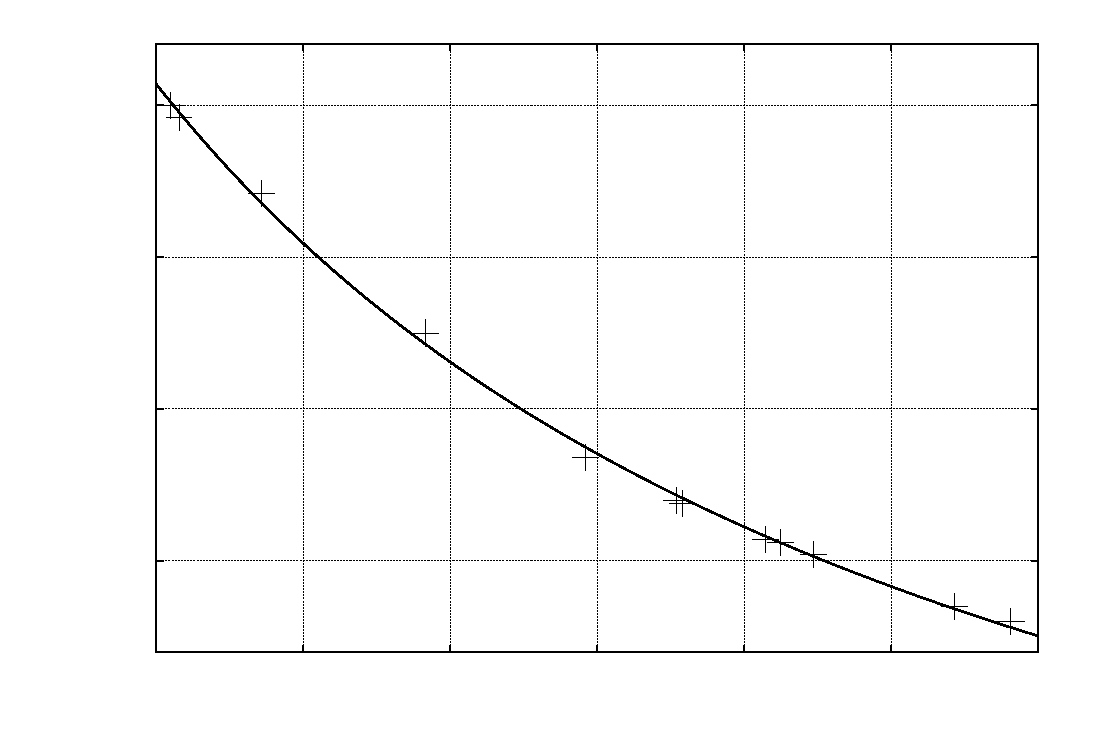
\includegraphics{hranol}}%
    \gplfronttext
  \end{picture}%
\endgroup

  \caption{Disperzní křivka skleněného hranolu}
  \label{g:h}
\end{graph}
\begin{graph}
  \centering
  % GNUPLOT: LaTeX picture with Postscript
\begingroup
  \makeatletter
  \providecommand\color[2][]{%
    \GenericError{(gnuplot) \space\space\space\@spaces}{%
      Package color not loaded in conjunction with
      terminal option `colourtext'%
    }{See the gnuplot documentation for explanation.%
    }{Either use 'blacktext' in gnuplot or load the package
      color.sty in LaTeX.}%
    \renewcommand\color[2][]{}%
  }%
  \providecommand\includegraphics[2][]{%
    \GenericError{(gnuplot) \space\space\space\@spaces}{%
      Package graphicx or graphics not loaded%
    }{See the gnuplot documentation for explanation.%
    }{The gnuplot epslatex terminal needs graphicx.sty or graphics.sty.}%
    \renewcommand\includegraphics[2][]{}%
  }%
  \providecommand\rotatebox[2]{#2}%
  \@ifundefined{ifGPcolor}{%
    \newif\ifGPcolor
    \GPcolorfalse
  }{}%
  \@ifundefined{ifGPblacktext}{%
    \newif\ifGPblacktext
    \GPblacktexttrue
  }{}%
  % define a \g@addto@macro without @ in the name:
  \let\gplgaddtomacro\g@addto@macro
  % define empty templates for all commands taking text:
  \gdef\gplbacktext{}%
  \gdef\gplfronttext{}%
  \makeatother
  \ifGPblacktext
    % no textcolor at all
    \def\colorrgb#1{}%
    \def\colorgray#1{}%
  \else
    % gray or color?
    \ifGPcolor
      \def\colorrgb#1{\color[rgb]{#1}}%
      \def\colorgray#1{\color[gray]{#1}}%
      \expandafter\def\csname LTw\endcsname{\color{white}}%
      \expandafter\def\csname LTb\endcsname{\color{black}}%
      \expandafter\def\csname LTa\endcsname{\color{black}}%
      \expandafter\def\csname LT0\endcsname{\color[rgb]{1,0,0}}%
      \expandafter\def\csname LT1\endcsname{\color[rgb]{0,1,0}}%
      \expandafter\def\csname LT2\endcsname{\color[rgb]{0,0,1}}%
      \expandafter\def\csname LT3\endcsname{\color[rgb]{1,0,1}}%
      \expandafter\def\csname LT4\endcsname{\color[rgb]{0,1,1}}%
      \expandafter\def\csname LT5\endcsname{\color[rgb]{1,1,0}}%
      \expandafter\def\csname LT6\endcsname{\color[rgb]{0,0,0}}%
      \expandafter\def\csname LT7\endcsname{\color[rgb]{1,0.3,0}}%
      \expandafter\def\csname LT8\endcsname{\color[rgb]{0.5,0.5,0.5}}%
    \else
      % gray
      \def\colorrgb#1{\color{black}}%
      \def\colorgray#1{\color[gray]{#1}}%
      \expandafter\def\csname LTw\endcsname{\color{white}}%
      \expandafter\def\csname LTb\endcsname{\color{black}}%
      \expandafter\def\csname LTa\endcsname{\color{black}}%
      \expandafter\def\csname LT0\endcsname{\color{black}}%
      \expandafter\def\csname LT1\endcsname{\color{black}}%
      \expandafter\def\csname LT2\endcsname{\color{black}}%
      \expandafter\def\csname LT3\endcsname{\color{black}}%
      \expandafter\def\csname LT4\endcsname{\color{black}}%
      \expandafter\def\csname LT5\endcsname{\color{black}}%
      \expandafter\def\csname LT6\endcsname{\color{black}}%
      \expandafter\def\csname LT7\endcsname{\color{black}}%
      \expandafter\def\csname LT8\endcsname{\color{black}}%
    \fi
  \fi
  \setlength{\unitlength}{0.0500bp}%
  \begin{picture}(10204.00,6802.00)%
    \gplgaddtomacro\gplbacktext{%
      \csname LTb\endcsname%
      \put(1210,1093){\makebox(0,0)[r]{\strut{} 1.328}}%
      \csname LTb\endcsname%
      \put(1210,1871){\makebox(0,0)[r]{\strut{} 1.33}}%
      \csname LTb\endcsname%
      \put(1210,2648){\makebox(0,0)[r]{\strut{} 1.332}}%
      \csname LTb\endcsname%
      \put(1210,3426){\makebox(0,0)[r]{\strut{} 1.334}}%
      \csname LTb\endcsname%
      \put(1210,4204){\makebox(0,0)[r]{\strut{} 1.336}}%
      \csname LTb\endcsname%
      \put(1210,4982){\makebox(0,0)[r]{\strut{} 1.338}}%
      \csname LTb\endcsname%
      \put(1210,5759){\makebox(0,0)[r]{\strut{} 1.34}}%
      \csname LTb\endcsname%
      \put(1210,6537){\makebox(0,0)[r]{\strut{} 1.342}}%
      \csname LTb\endcsname%
      \put(1342,484){\makebox(0,0){\strut{} 400}}%
      \csname LTb\endcsname%
      \put(2753,484){\makebox(0,0){\strut{} 450}}%
      \csname LTb\endcsname%
      \put(4164,484){\makebox(0,0){\strut{} 500}}%
      \csname LTb\endcsname%
      \put(5575,484){\makebox(0,0){\strut{} 550}}%
      \csname LTb\endcsname%
      \put(6985,484){\makebox(0,0){\strut{} 600}}%
      \csname LTb\endcsname%
      \put(8396,484){\makebox(0,0){\strut{} 650}}%
      \csname LTb\endcsname%
      \put(9807,484){\makebox(0,0){\strut{} 700}}%
      \put(176,3620){\rotatebox{-270}{\makebox(0,0){\strut{}$n$}}}%
      \put(5574,154){\makebox(0,0){\strut{}$\lambda$ (\si{\nm})}}%
    }%
    \gplgaddtomacro\gplfronttext{%
    }%
    \gplbacktext
    \put(0,0){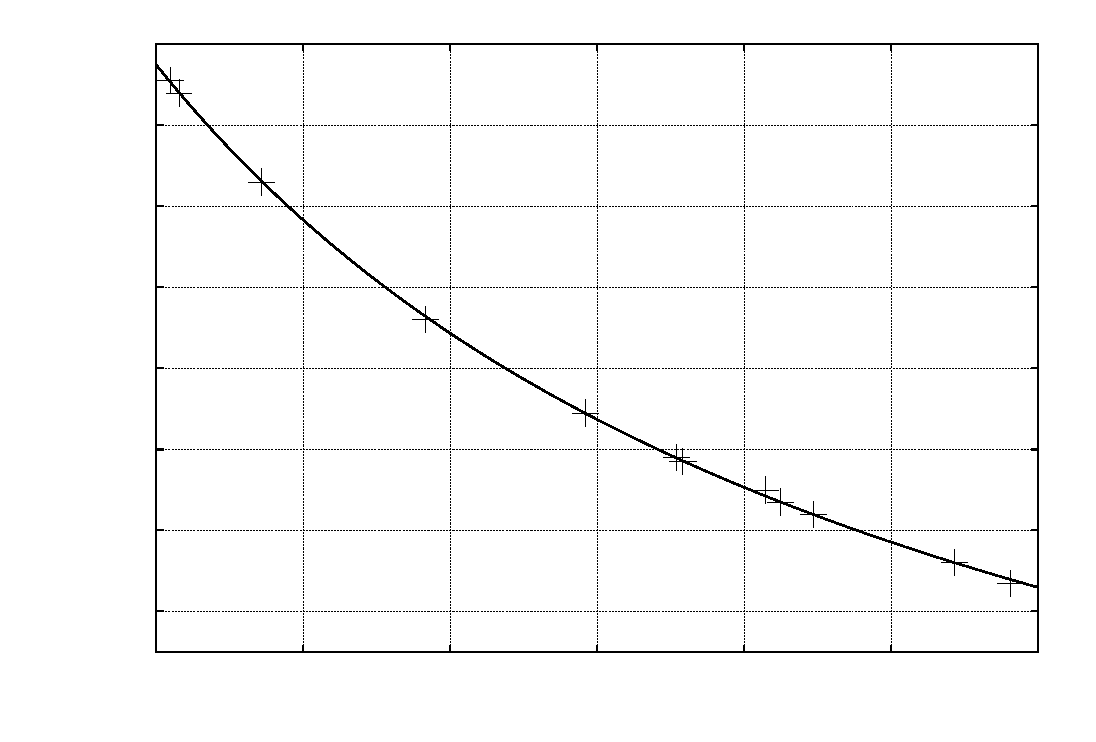
\includegraphics{kap}}%
    \gplfronttext
  \end{picture}%
\endgroup

  \caption{Disperzní křivka kapaliny v kyvetě}
  \label{g:k}
\end{graph}

Spočetli jsme střední disperzi, relativní disperzi a Abbeovo číslo pro hranol (s indexem h) a kapalinu (s indexem k)
\begin{equation} \label{e:vysledky}
\begin{array}{rclrclrcl}
\Delta_h &= &\num{0.0100(1)} \qquad \qquad &\delta_h &= &\num{0.019(1)} \qquad \qquad &\gamma_h &= &\num{51(2)} \\
\Delta_k &= &\num{0.0070(1)} \qquad \qquad &\delta_k &= &\num{0.021(1)} \qquad \qquad &\gamma_k &= &\num{47(2)}
\end{array}
\end{equation}